\documentclass[tikz,border=2pt]{standalone}
\usepackage{pgfplots}
\pgfplotsset{compat=1.18}

\begin{document}
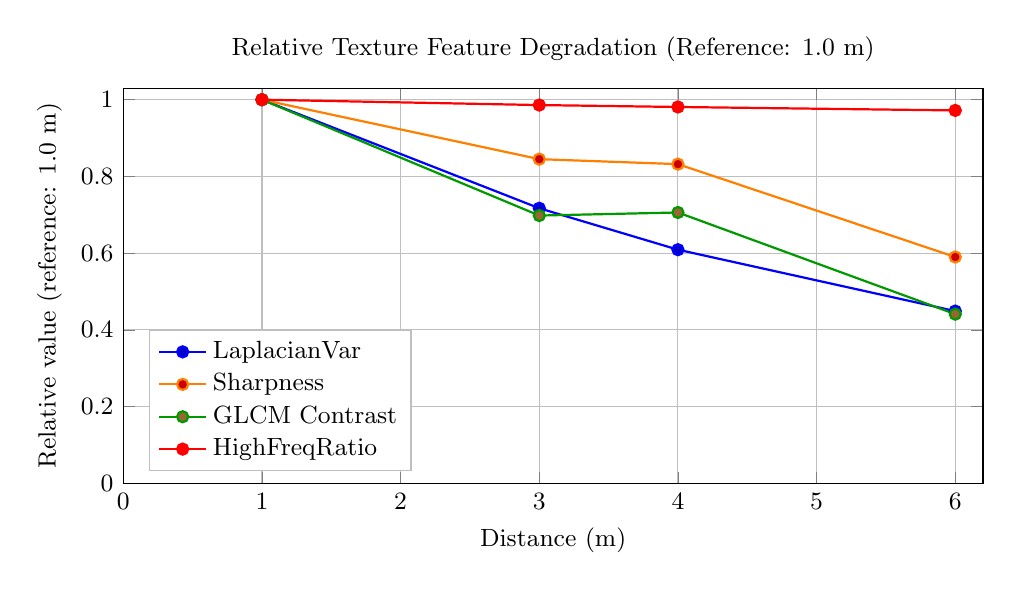
\begin{tikzpicture}
\begin{axis}[
  width=12.5cm,
  height=6.6cm,
  xlabel={Distance (m)},
  ylabel={Relative value (reference: 1.0 m)},
  xmin=0, xmax=6.2,
  ymin=0, ymax=1.03,
  xtick={0,1,2,3,4,5,6},
  ytick={0,0.2,0.4,0.6,0.8,1.0},
  grid=major,
  legend pos=south west,
  legend cell align=left,
  tick label style={font=\small},
  label style={font=\small},
  legend style={font=\small, fill=white, draw=black!25},
  title={Relative Texture Feature Degradation (Reference: 1.0 m)},
  title style={font=\small}
]
\addplot+[blue, mark=*, line width=0.8pt] coordinates {(1,1.000) (3,0.717) (4,0.609) (6,0.449)};
\addlegendentry{LaplacianVar}
\addplot+[orange, mark=*, line width=0.8pt] coordinates {(1,1.000) (3,0.845) (4,0.832) (6,0.590)};
\addlegendentry{Sharpness}
\addplot+[green!60!black, mark=*, line width=0.8pt] coordinates {(1,1.000) (3,0.698) (4,0.706) (6,0.441)};
\addlegendentry{GLCM Contrast}
\addplot+[red, mark=*, line width=0.8pt] coordinates {(1,1.000) (3,0.986) (4,0.981) (6,0.972)};
\addlegendentry{HighFreqRatio}
\end{axis}
\end{tikzpicture}
\end{document}
